\documentclass[12pt, a4paper]{article}

% --- Packages ---
\usepackage[utf8]{inputenc}
\usepackage[T1]{fontenc}
\usepackage{geometry}
\geometry{a4paper, margin=1in, headheight=15pt}
\usepackage{xcolor}
\usepackage{hyperref}
\usepackage{graphicx}
\usepackage{tcolorbox}
\usepackage{fancyhdr}
\usepackage{titlesec}
\usepackage{enumitem}
\usepackage{parskip}
\usepackage{caption}
\usepackage{float}
\usepackage{listings}

% --- Colors ---
\definecolor{primary}{RGB}{12, 74, 110}     % Dark Slate Blue
\definecolor{secondary}{RGB}{2, 132, 199}   % Sky Blue
\definecolor{accent}{RGB}{240, 249, 255}    % Very Light Blue for backgrounds
\definecolor{darkgray}{RGB}{71, 85, 105}
\definecolor{codebg}{RGB}{248, 250, 252}

% --- Hyperref Setup ---
\hypersetup{
    colorlinks=true,
    linkcolor=primary,
    filecolor=secondary,      
    urlcolor=secondary,
    pdftitle={Comprehensive Week 4 Report - CalderR Internship},
    pdfpagemode=FullScreen,
}

% --- Header and Footer Setup ---
\pagestyle{fancy}
\fancyhf{}
\rhead{\textcolor{darkgray}{\textbf{Week 4 Comprehensive Report}}}
\lhead{\textcolor{darkgray}{CalderR Agentic AI Internship, 2026}}
\cfoot{\textcolor{darkgray}{Page \thepage}}
\renewcommand{\headrulewidth}{0.4pt}
\renewcommand{\footrulewidth}{0.4pt}

% --- Section Formatting ---
\titleformat{\section}
  {\LARGE\bfseries\color{primary}}{\thesection}{1em}{}[{\titlerule[1.2pt]}]

\titleformat{\subsection}
  {\Large\bfseries\color{secondary}}{\thesubsection}{1em}{}

\titleformat{\subsubsection}
  {\large\bfseries\color{primary}}{\thesubsubsection}{1em}{}

% --- Document Starts Here ---
\begin{document}

% --- Title Page ---
\begin{titlepage}
    \centering
    \vspace*{2cm}
    
    {\Huge \textbf{\textcolor{primary}{Agentic AI Engineering Internship}}} \\[0.5cm]
    {\Huge \textbf{\textcolor{primary}{2026}}} \\[1.5cm]
    
    {\LARGE \textbf{Week 4 Comprehensive Report}} \\[0.5cm]
    {\Large \textit{LangGraph, Workflows \& State Machines}} \\[2cm]
    
    \begin{tcolorbox}[colback=accent, colframe=primary, rounded corners, boxrule=1.5pt, width=0.75\textwidth, arc=4mm]
        \centering
        \vspace{0.4cm}
        {\Large \textbf{Prepared By:}} \\[0.2cm]
        {\Large \textbf{Ghafoor}} \\[0.4cm]
        {\large \textbf{Date:}} \\
        {\large \today}
        \vspace{0.4cm}
    \end{tcolorbox}
    
    \vfill
    
    {\huge \textbf{\textcolor{secondary}{CalderR.}}} \\[0.2cm]
    {\large \textit{RETHINKING $\cdot$ HOW $\cdot$ WORK $\cdot$ WORKS}}
    \vspace*{1cm}
\end{titlepage}

% --- Table of Contents ---
\tableofcontents
\newpage

% --- Section 1: Executive Summary ---
\section{Executive Summary}
This comprehensive report documents the theoretical learnings, hands-on labs, and advanced architectural implementations completed during Week 4 of the CalderR Agentic AI Engineering Internship. Transitioning from linear chains to graph-based orchestration, the focus of the week was mastering LangGraph's node-edge-state model. The core objective was to build sophisticated stateful agents capable of branching, looping, pausing for human approval, and persisting state across sessions. These foundational skills are critical for orchestrating complex AI flows.

The week culminated in the successful deployment of two advanced projects: a \textbf{Customer Onboarding Agent} (Intermediate) and an \textbf{AI-Powered Hiring Pipeline} (Production). These projects synthesized the week's learnings by implementing multi-step workflows, conditional routing, human-in-the-loop (HITL) approval gates, state persistence, bias detection, and audit logging.

% --- Section 2: Conceptual Mastery & Assessment ---
\section{Conceptual Mastery \& Assessment}
The curriculum emphasized transitioning into graph-based orchestration for stateful and resilient agent workflows.

\subsection{LangGraph, Workflows \& State Machines}
\begin{itemize}[label=\textcolor{secondary}{$\bullet$}]
    \item \textbf{LangGraph Core \& State Management:} Explored the \texttt{StateGraph} architecture, leveraging nodes, edges, and conditional routing. Mastered \texttt{TypedDict} state schemas and \texttt{Annotated} reducers for managing message histories and partial state updates across iterations.
    \item \textbf{Graph Patterns \& Iterative Refinement:} Moved beyond simple pipelines to build branching, looping, and parallel execution patterns. Implemented self-correcting agent loops that validate output and regenerate dynamically.
    \item \textbf{Human-in-the-Loop \& Persistence:} Engineered interrupt patterns using \texttt{SqliteSaver} and checkpointers to pause execution for human review, persisting the state across sessions, and resuming workflows seamlessly after approval.
    \item \textbf{Streaming \& Debugging:} Utilized LangSmith for deep tracing, step-by-step debugging, and visualization of complex graph states and conditional execution paths.
\end{itemize}

\newpage

% --- Section 3: Production Project ---
\section{Production Project: AI-Powered Hiring Pipeline}

\begin{tcolorbox}[colback=accent, colframe=primary, title=\textbf{Architectural Overview}, boxrule=1pt]
A complete hiring workflow built with FastAPI and LangGraph. It ingests resumes, scores them against job descriptions, checks for biases, shortlists candidates, generates interview questions, and incorporates a human-in-the-loop (HITL) review stage for final decisions. It features a robust audit log stored in SQLite to track all state transitions and decisions.
\end{tcolorbox}

\begin{figure}[H]
    \centering
    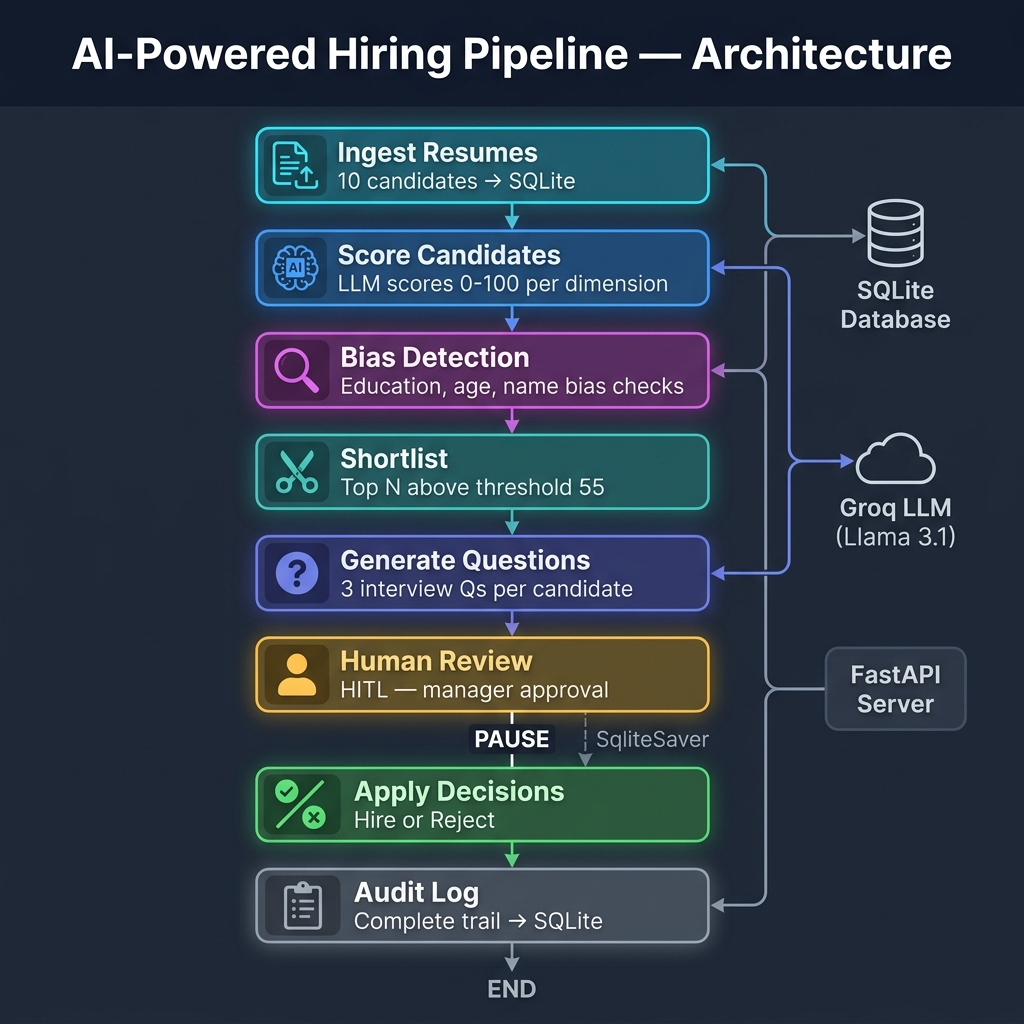
\includegraphics[width=0.85\textwidth]{projects/hiring_pipeline/architecture_diagram.png}
    \caption{Production Project: Complete System Architecture}
\end{figure}

\subsection{Technical Implementation}
\begin{itemize}[label=\textcolor{secondary}{$\bullet$}]
    \item \textbf{Complex Graph Orchestration:} Engineered a sophisticated LangGraph workflow with multiple nodes and conditional edges to accurately route candidates through scoring, bias detection, and shortlisting stages.
    \item \textbf{Human-in-the-Loop Integration:} Implemented checkpointers to pause the pipeline for manual review of shortlisted candidates before proceeding to final interview question generation and decisions.
    \item \textbf{Audit Logging \& Persistence:} Integrated SQLite for persistent audit logging of state transitions, scoring metrics, and manual approvals, ensuring a transparent and traceable hiring workflow.
\end{itemize}

\subsection{System Demonstrations}
\begin{figure}[H]
    \centering
    \begin{minipage}{0.48\textwidth}
        \centering
        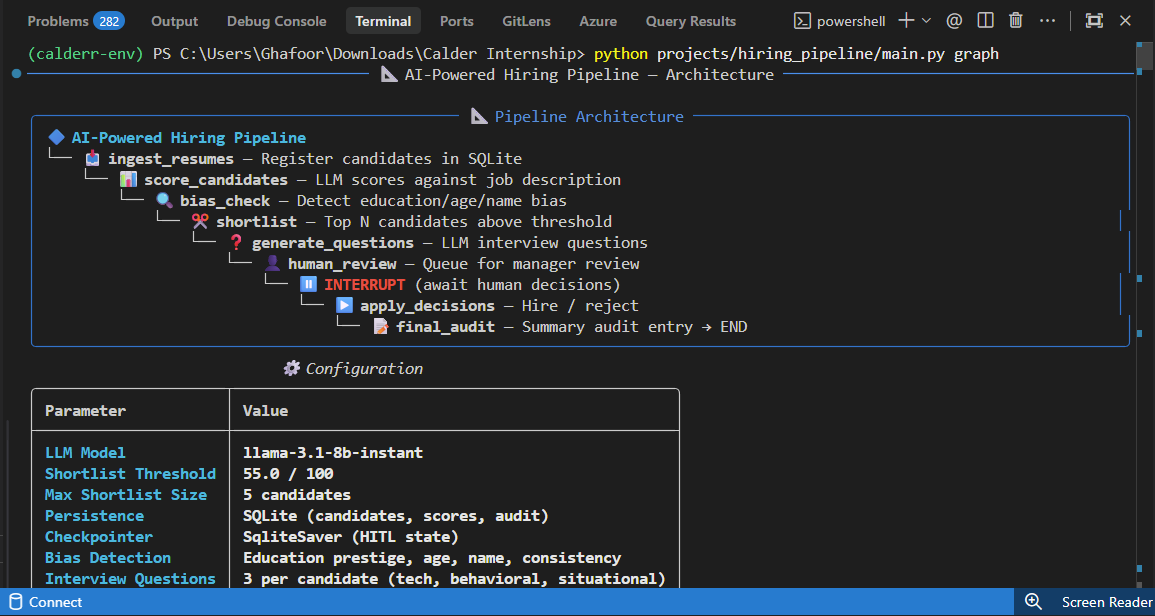
\includegraphics[width=\linewidth, keepaspectratio]{screenshots/Week4/Prod-1.png}
        \caption{Pipeline Architecture \& Configuration}
    \end{minipage}\hfill
    \begin{minipage}{0.48\textwidth}
        \centering
        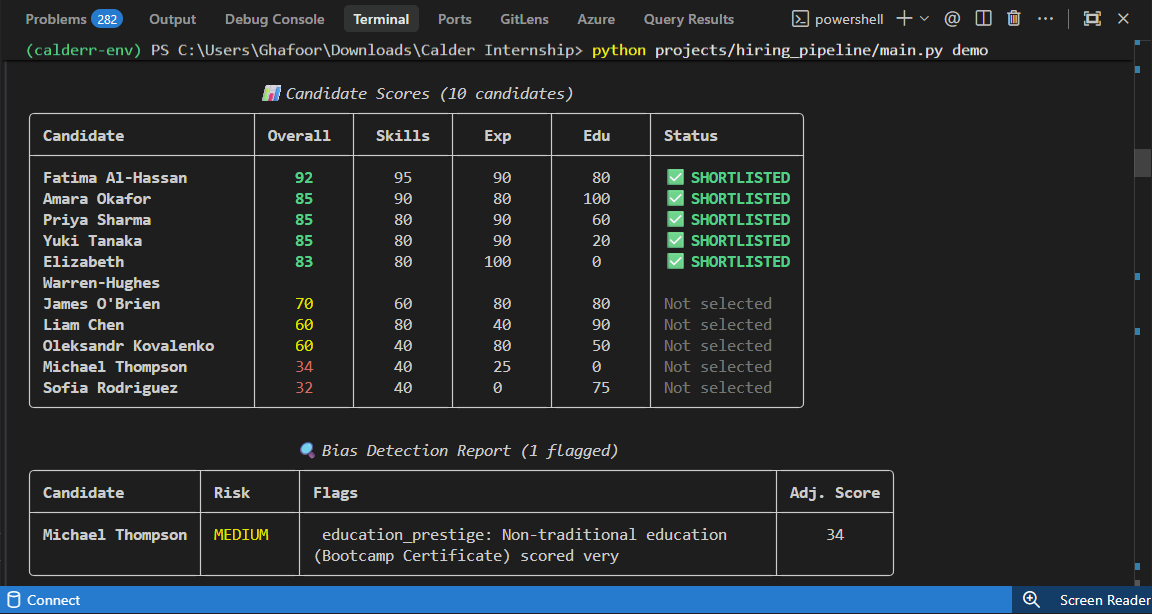
\includegraphics[width=\linewidth, keepaspectratio]{screenshots/Week4/Prod-2.png}
        \caption{Candidate Scoring \& Evaluation}
    \end{minipage}
\end{figure}

\begin{figure}[H]
    \centering
    \begin{minipage}{0.48\textwidth}
        \centering
        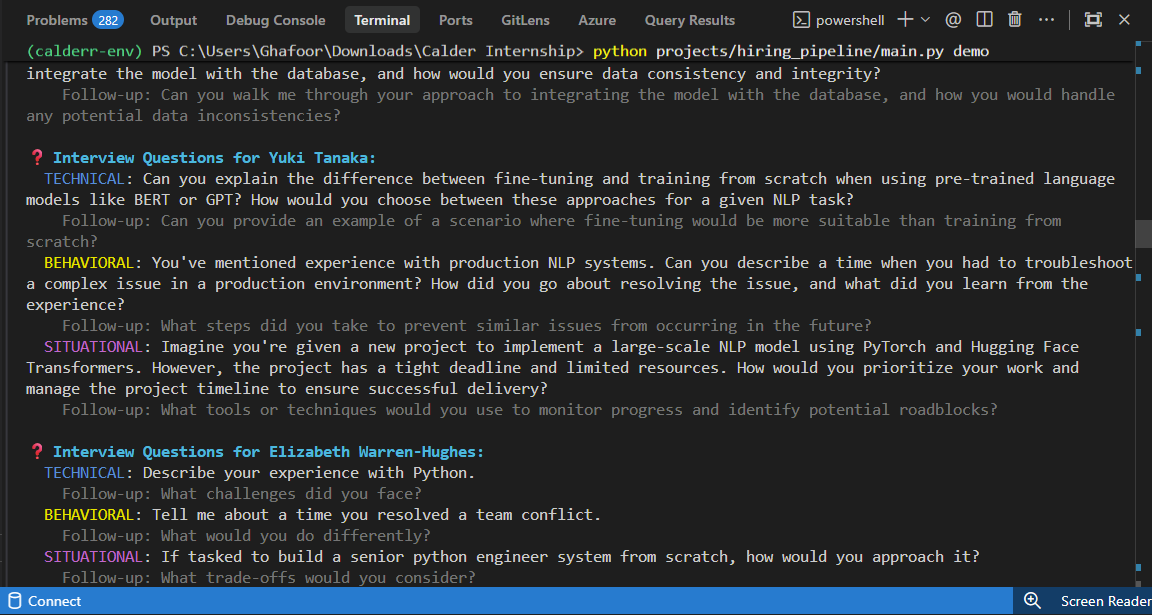
\includegraphics[width=\linewidth, keepaspectratio]{screenshots/Week4/Prod-3.png}
        \caption{Candidates Interview Questioning}
    \end{minipage}\hfill
    \begin{minipage}{0.48\textwidth}
        \centering
        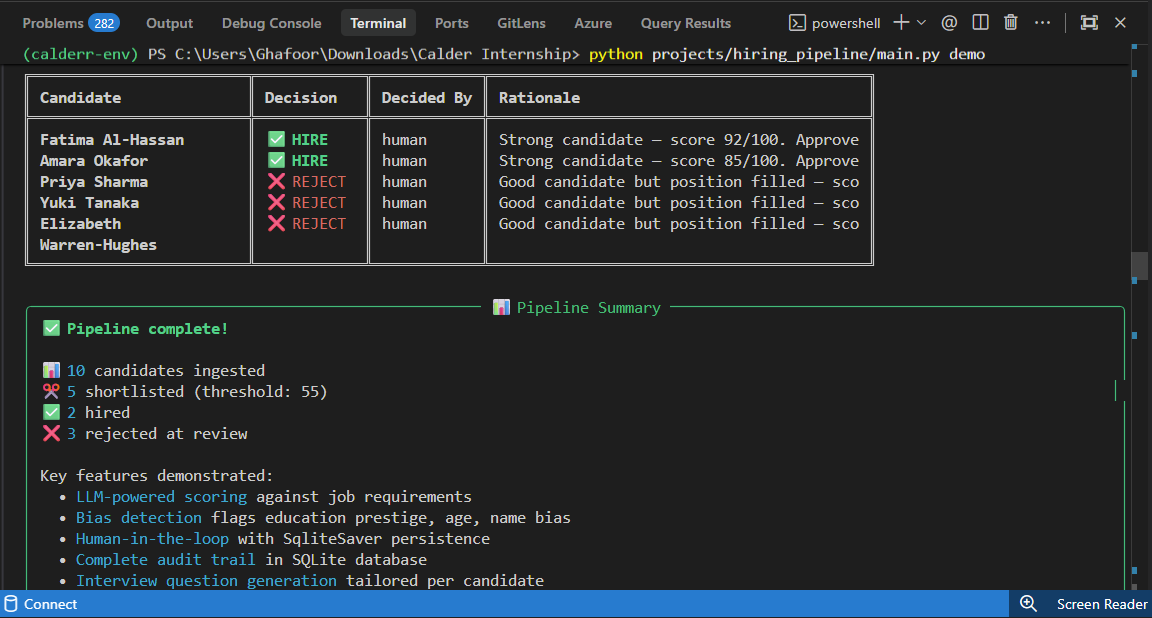
\includegraphics[width=\linewidth, keepaspectratio]{screenshots/Week4/Prod-4.png}
        \caption{Human-in-the-Loop Review Dashboard}
    \end{minipage}
\end{figure}

\begin{figure}[H]
    \centering
    \begin{minipage}{0.48\textwidth}
        \centering
        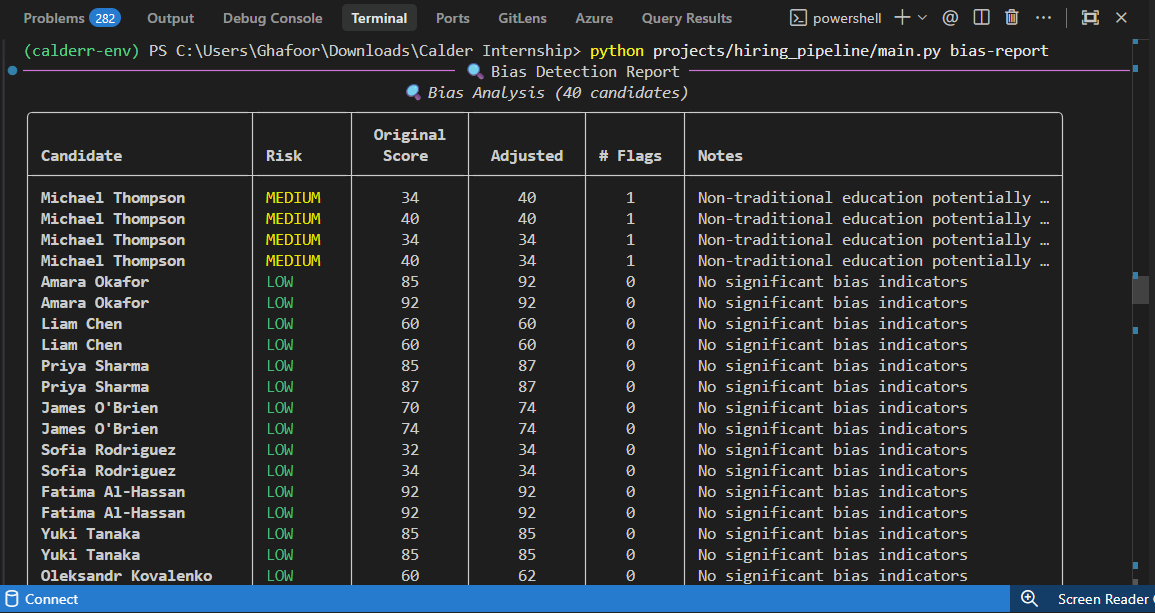
\includegraphics[width=\linewidth, keepaspectratio]{screenshots/Week4/Prod-5.png}
        \caption{Bias Detection Report}
    \end{minipage}\hfill
    \begin{minipage}{0.48\textwidth}
        \centering
        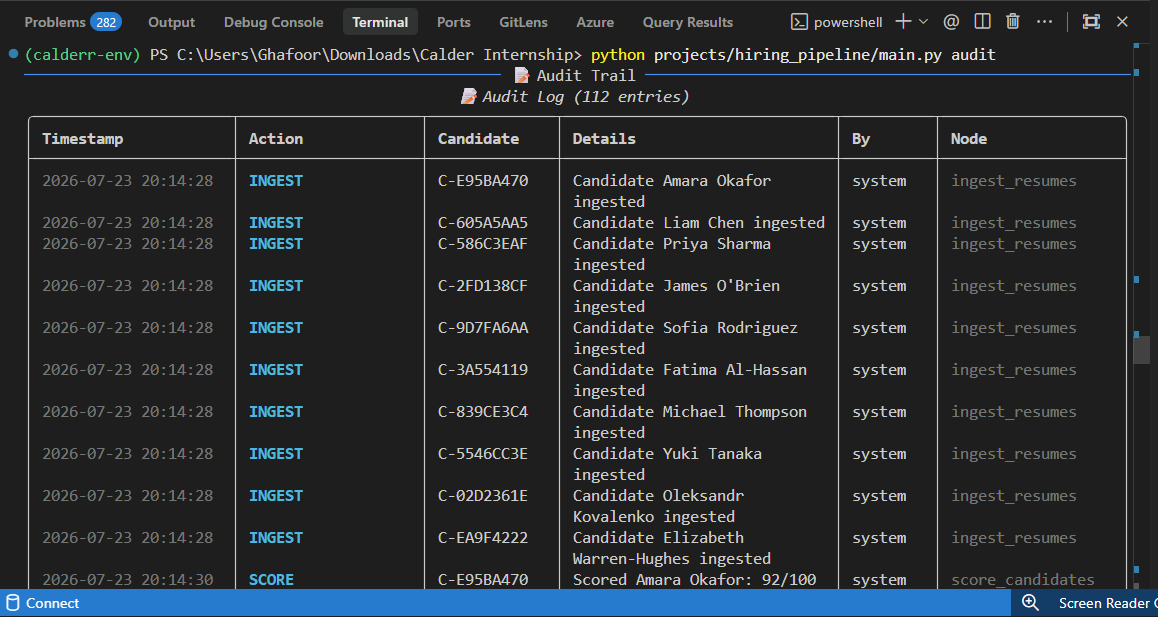
\includegraphics[width=\linewidth, keepaspectratio]{screenshots/Week4/Prod-6.png}
        \caption{Audit Log \& Trail}
    \end{minipage}
\end{figure}

\begin{figure}[H]
    \centering
    \begin{minipage}{0.5\textwidth}
        \centering
        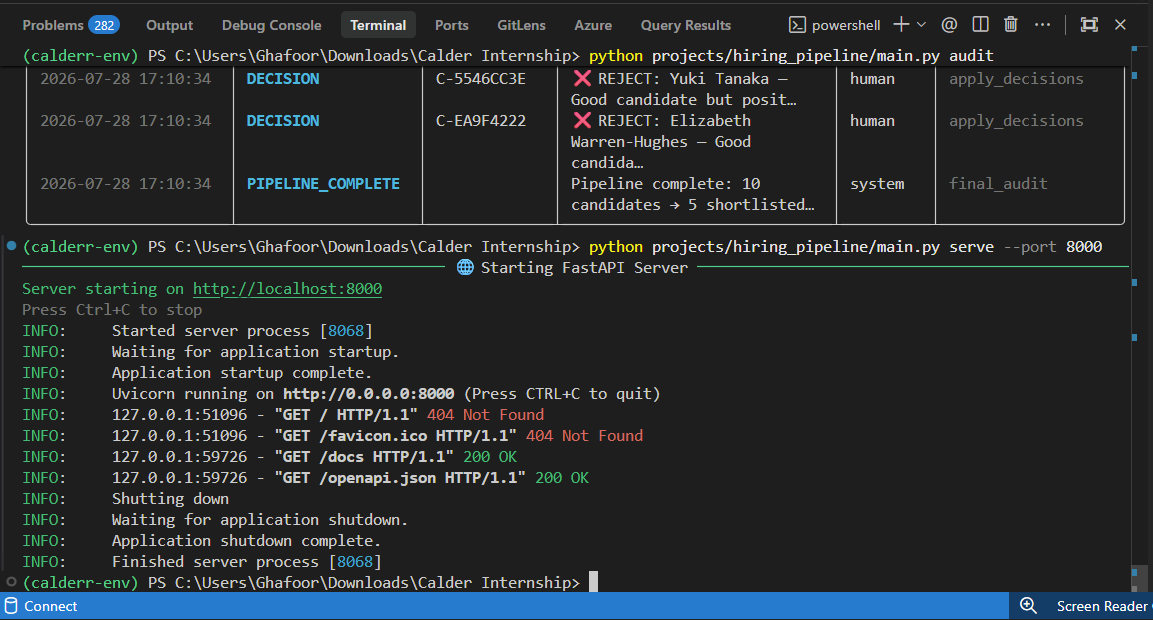
\includegraphics[width=\linewidth, keepaspectratio]{screenshots/Week4/Prod-7.png}
        \caption{FastAPI Server Endpoints}
    \end{minipage}
\end{figure}

\newpage

% --- Section 4: Intermediate Project ---
\section{Intermediate Project: Customer Onboarding Agent}

\begin{tcolorbox}[colback=accent, colframe=primary, title=\textbf{Architectural Overview}, boxrule=1pt]
A multi-step onboarding workflow that collects customer information, validates it, and generates accounts. It dynamically routes standard accounts for auto-approval while requiring human review for large accounts, demonstrating robust conditional routing and state persistence.
\end{tcolorbox}

\begin{figure}[H]
    \centering
    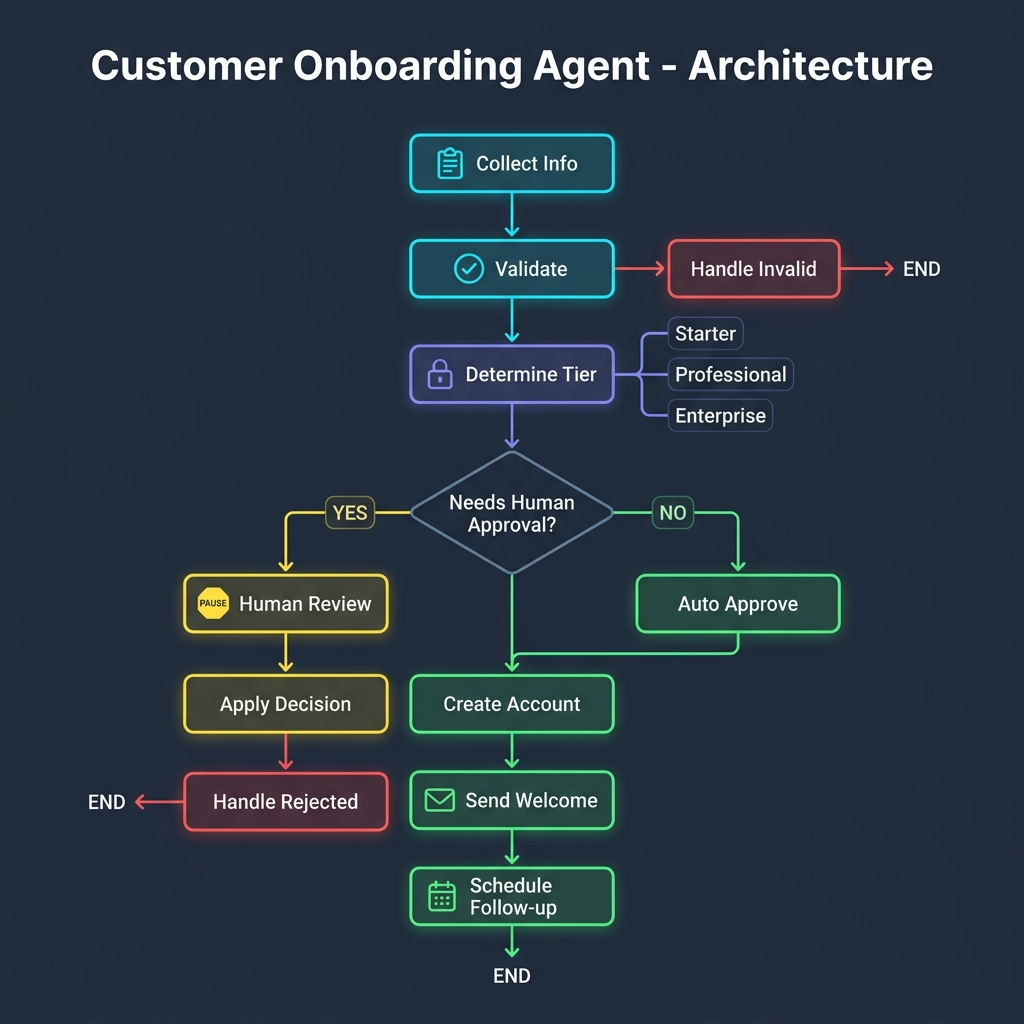
\includegraphics[width=0.85\textwidth]{projects/customer_onboarding/architecture_diagram.png}
    \caption{Intermediate Project: Multi-step Workflow Architecture}
\end{figure}

\subsection{Technical Implementation}
\begin{itemize}[label=\textcolor{secondary}{$\bullet$}]
    \item \textbf{Conditional Routing:} Utilized conditional edges to route standard vs. large accounts to entirely different approval nodes, demonstrating complex decision logic.
    \item \textbf{State Persistence \& Interruption:} Implemented state persistence to allow the human review node to interrupt the workflow and resume cleanly upon a manual decision, maintaining all collected data.
    \item \textbf{Multi-Step Pipeline:} Orchestrated sequential nodes for info collection, validation, account creation, and automated follow-up scheduling.
\end{itemize}

\subsection{System Demonstrations}
\begin{figure}[H]
    \centering
    \begin{minipage}{0.48\textwidth}
        \centering
        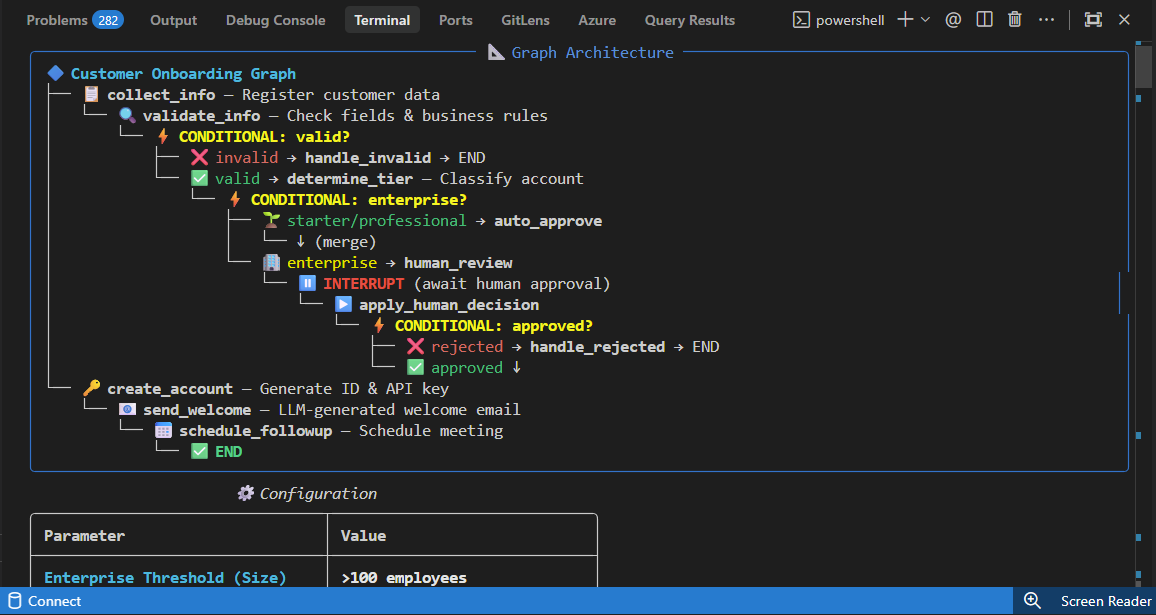
\includegraphics[width=\linewidth, keepaspectratio]{screenshots/Week4/Inter-1.png}
        \caption{Graph Architecture \& Configuration}
    \end{minipage}\hfill
    \begin{minipage}{0.48\textwidth}
        \centering
        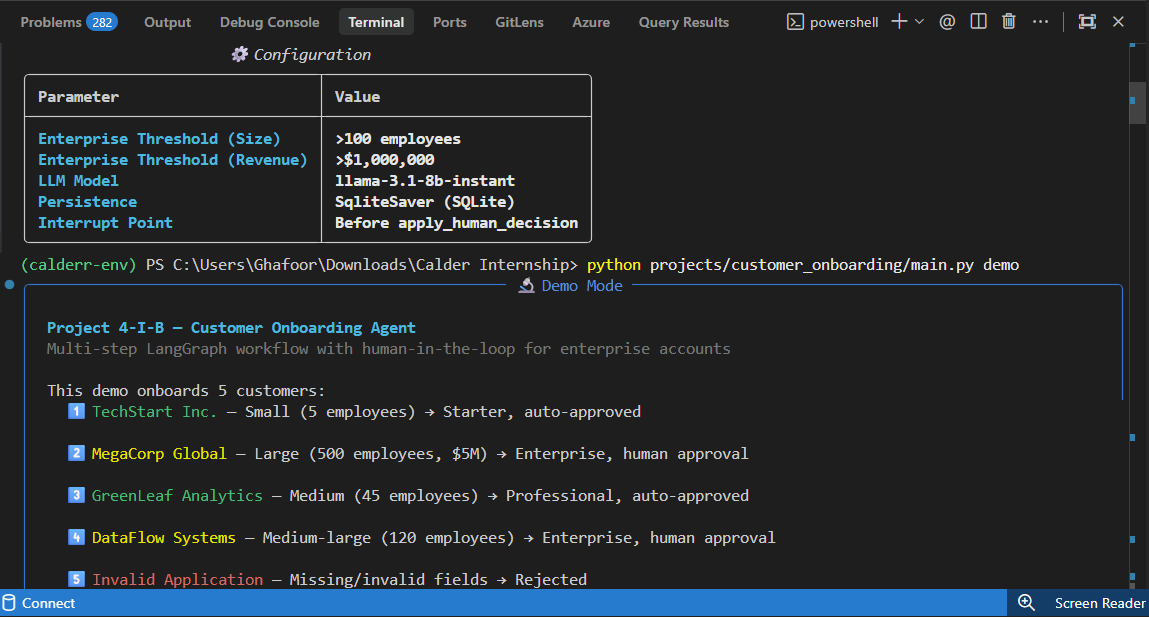
\includegraphics[width=\linewidth, keepaspectratio]{screenshots/Week4/Inter-2.png}
        \caption{Information Collection \& Validation}
    \end{minipage}
\end{figure}

\vspace{0.3cm}

\begin{figure}[H]
    \centering
    \begin{minipage}{0.48\textwidth}
        \centering
        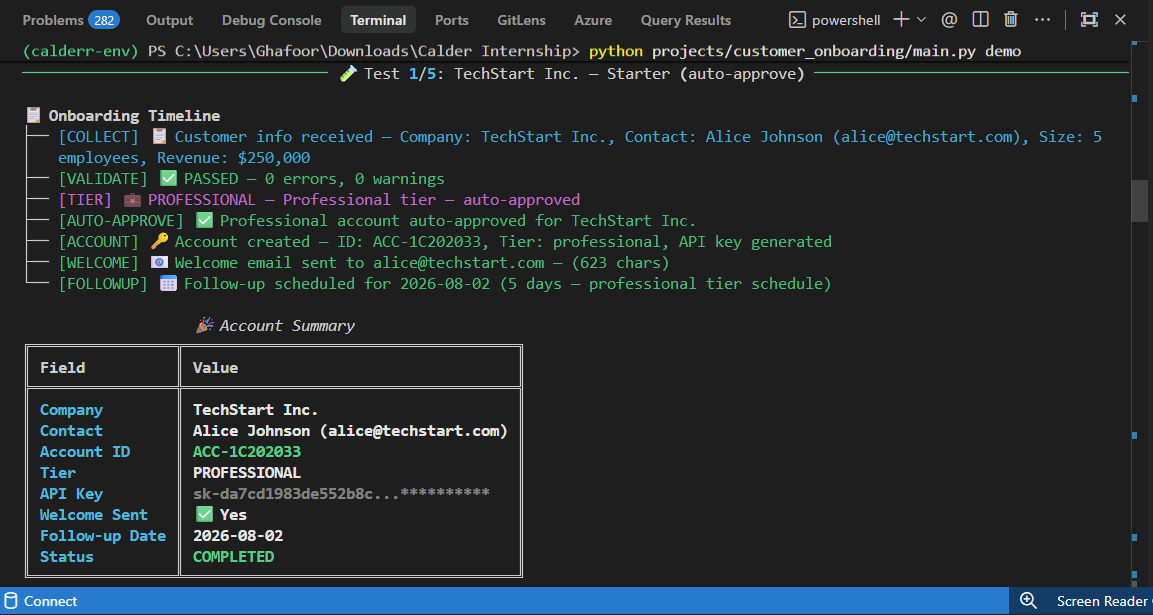
\includegraphics[width=\linewidth, keepaspectratio]{screenshots/Week4/Inter-3.png}
        \caption{Conditional Routing by Account Size}
    \end{minipage}\hfill
    \begin{minipage}{0.48\textwidth}
        \centering
        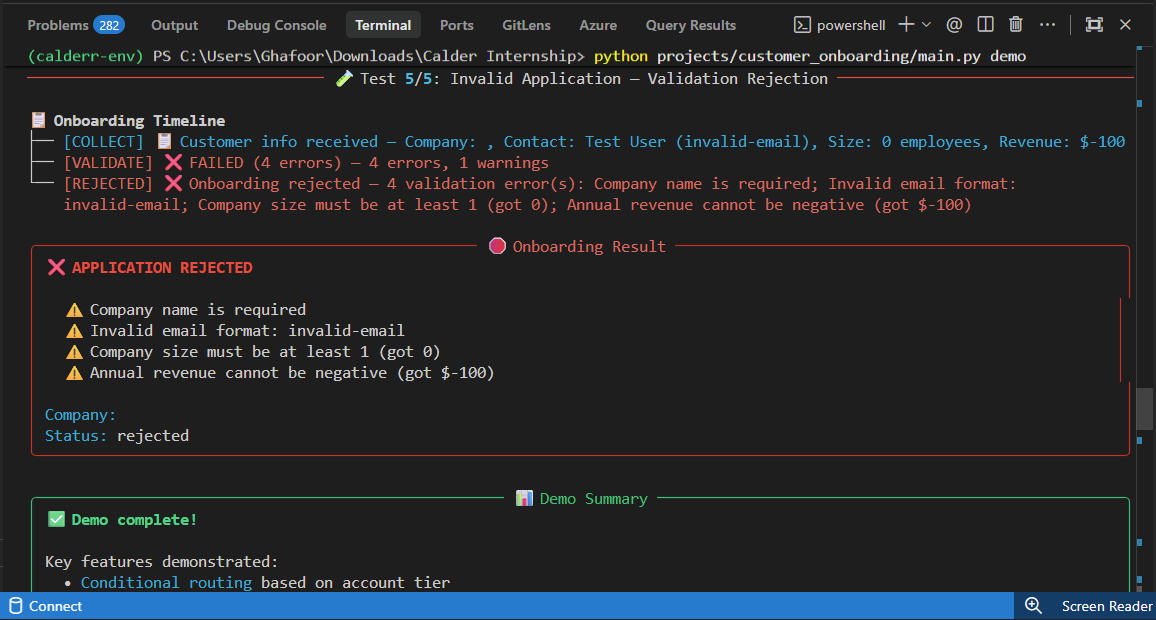
\includegraphics[width=\linewidth, keepaspectratio]{screenshots/Week4/Inter-4.png}
        \caption{Information Collection \& Validation}
    \end{minipage}
\end{figure}

\begin{figure}[H]
    \centering
    \begin{minipage}{0.48\textwidth}
        \centering
        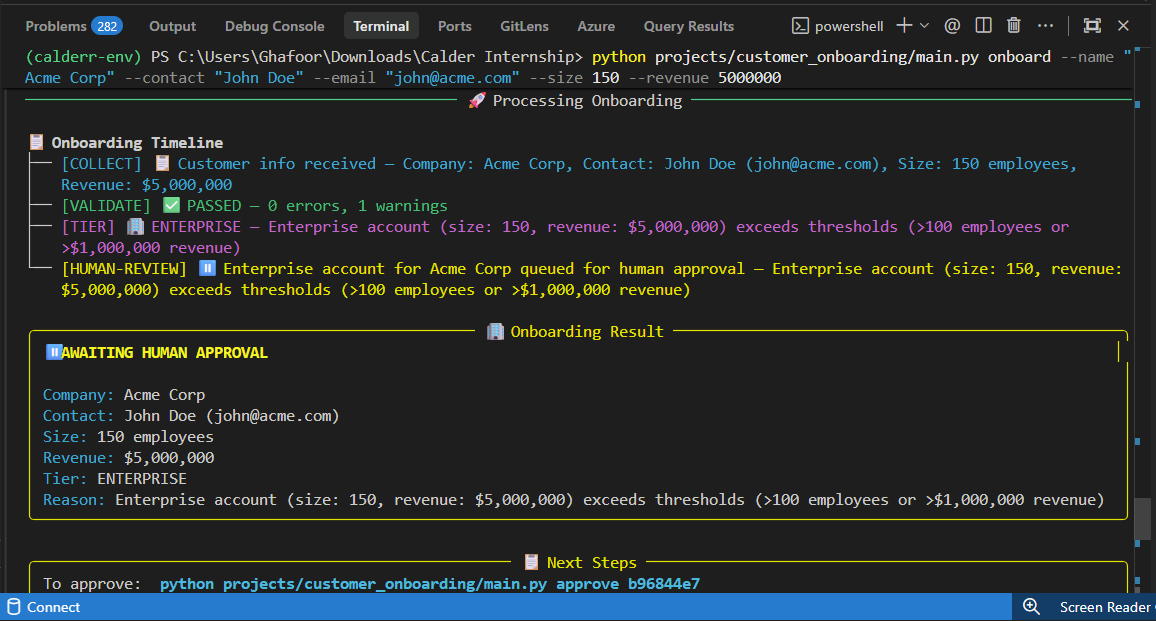
\includegraphics[width=\linewidth, keepaspectratio]{screenshots/Week4/Inter-5.png}
        \caption{Awaiting Human Approval for Account}
    \end{minipage}\hfill
    \begin{minipage}{0.48\textwidth}
        \centering
        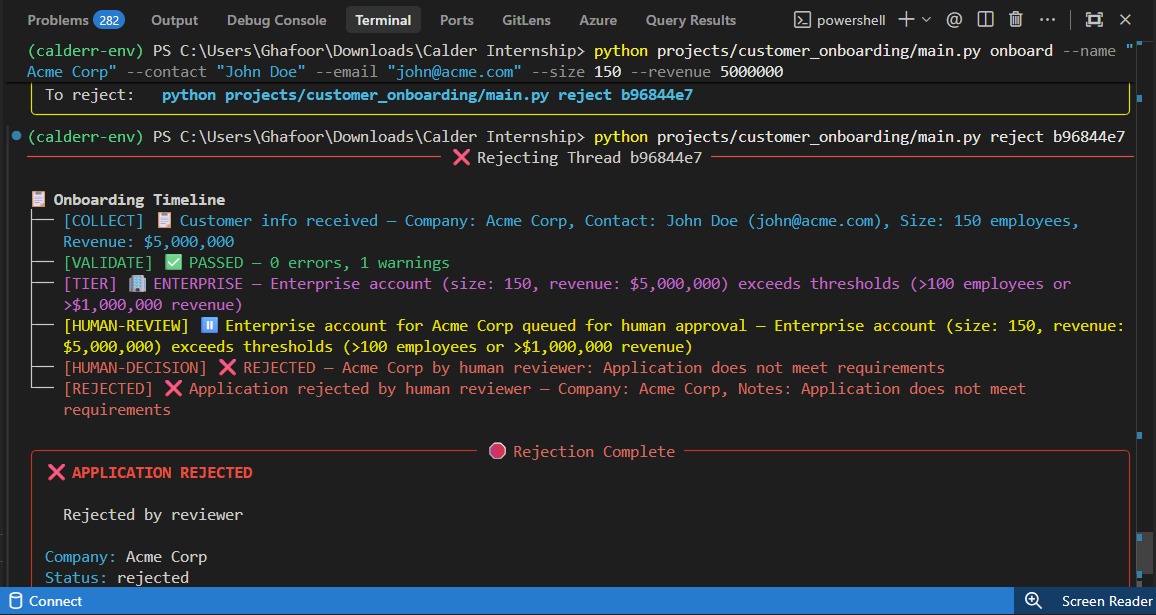
\includegraphics[width=\linewidth, keepaspectratio]{screenshots/Week4/Inter-6.png}
        \caption{Application Rejection}
    \end{minipage}
\end{figure}

\newpage

% --- Section 5: Foundational Labs ---
\section{Foundational Labs Deep-Dive}

\subsection{Lab 4.1: Document Processing Graph}
Built a foundational LangGraph workflow featuring a load $\rightarrow$ validate $\rightarrow$ chunk $\rightarrow$ embed $\rightarrow$ confirm pipeline.
\begin{itemize}[label=\textcolor{secondary}{$\bullet$}]
    \item \textbf{Conditional Splitting:} Added a conditional edge so that oversized documents are automatically routed to a splitting node before continuing.
    \item \textbf{Graph Compilation:} Visualized the \texttt{StateGraph} compilation and verified proper routing of documents through the embedding pipeline.
\end{itemize}

\begin{figure}[H]
    \centering
    \begin{minipage}{0.48\textwidth}
        \centering
        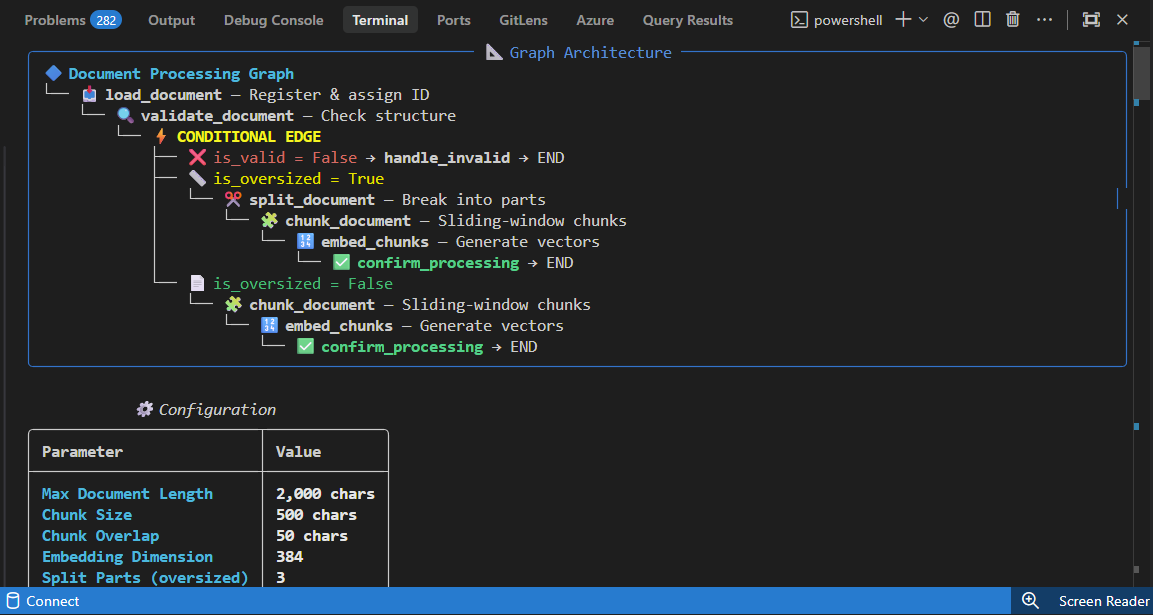
\includegraphics[width=\linewidth]{screenshots/Week4/Lab4.1-1.png}
        \caption{Graph Compilation \& Node Setup}
    \end{minipage}\hfill
    \begin{minipage}{0.48\textwidth}
        \centering
        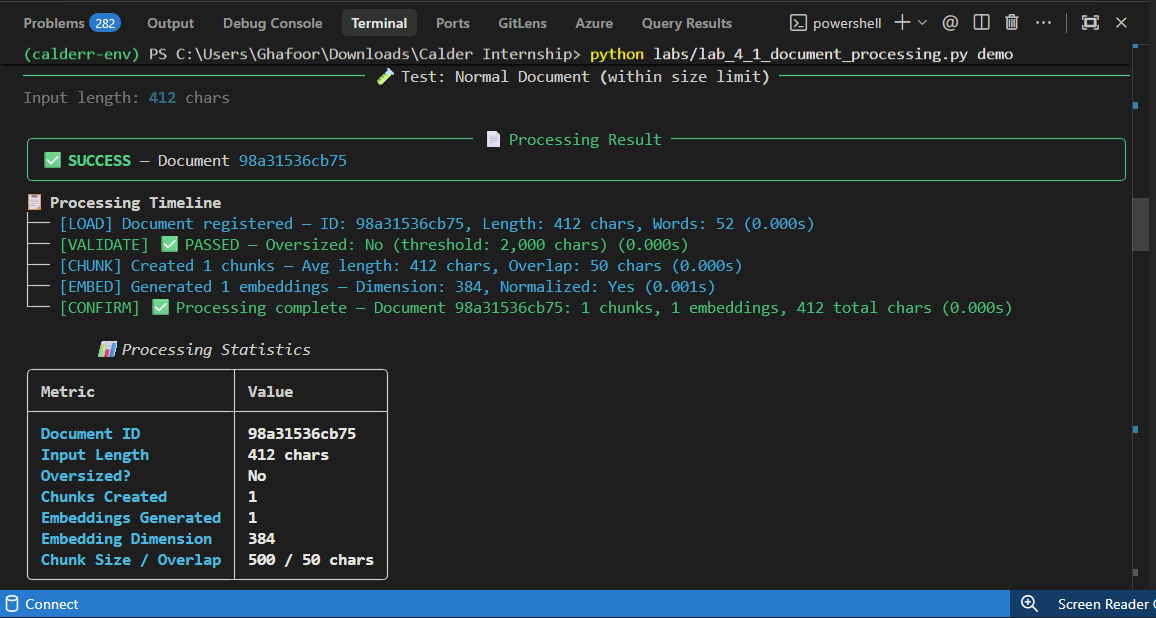
\includegraphics[width=\linewidth]{screenshots/Week4/Lab4.1-2.png}
        \caption{Document Loading \& Validation}
    \end{minipage}
\end{figure}

\begin{figure}[H]
    \centering
    \begin{minipage}{0.48\textwidth}
        \centering
        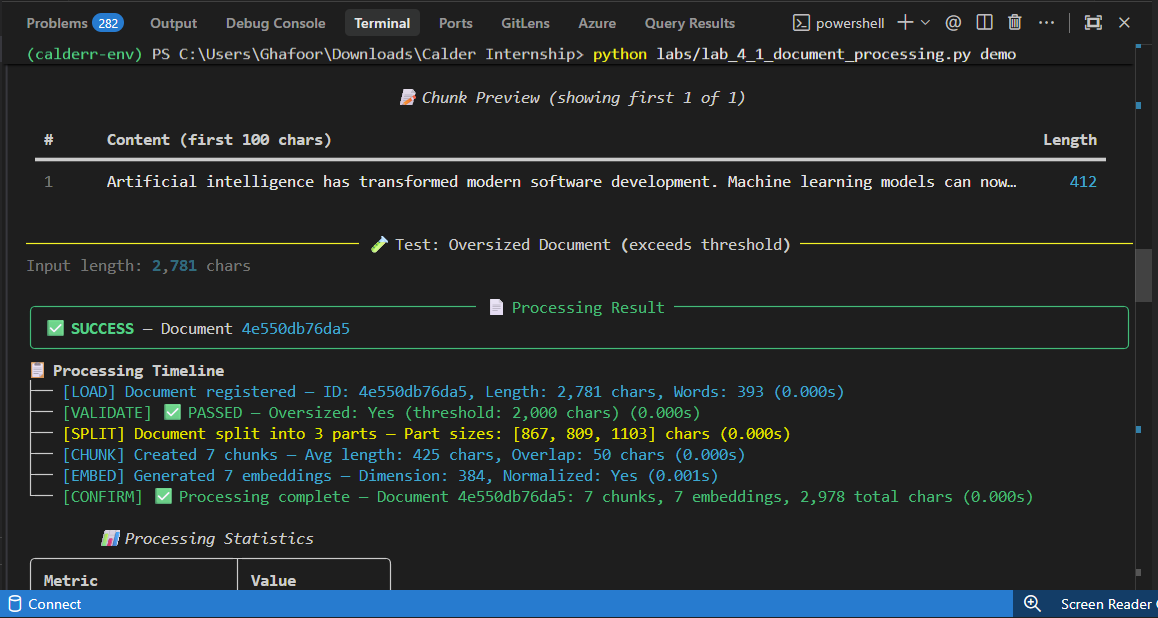
\includegraphics[width=\linewidth]{screenshots/Week4/Lab4.1-3.png}
        \caption{Embedding \& Confirmation}
    \end{minipage}\hfill
    \begin{minipage}{0.48\textwidth}
        \centering
        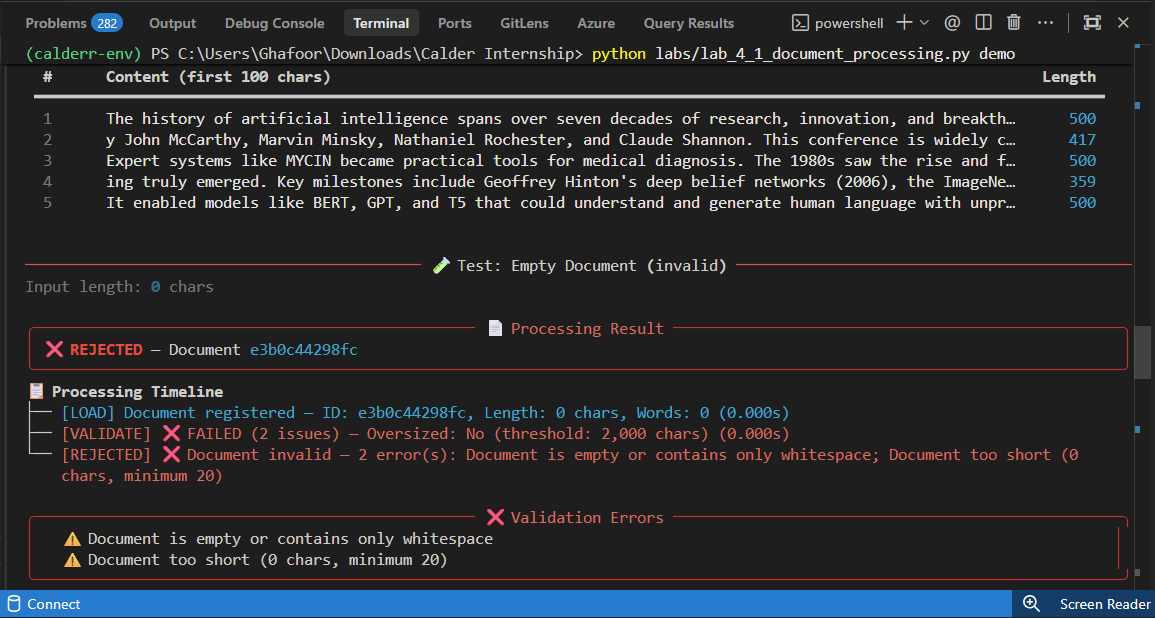
\includegraphics[width=\linewidth]{screenshots/Week4/Lab4.1-4.png}
        \caption{Document Validation \& Result}
    \end{minipage}
\end{figure}

\vspace{0.5cm}

\subsection{Lab 4.2: Self-Correcting Agent Loop}
Implemented a cyclic graph capable of self-correction through iterative refinement and validation.
\begin{itemize}[label=\textcolor{secondary}{$\bullet$}]
    \item \textbf{Bounded Retries:} Built a generate $\rightarrow$ validate $\rightarrow$ respond/regenerate loop that safely retries up to 3 times upon validation failure.
    \item \textbf{Iteration Tracking:} Developed state reducers to correctly track and log the number of iterations required for successful output.
\end{itemize}

\begin{figure}[H]
    \centering
    \begin{minipage}{0.31\textwidth}
        \centering
        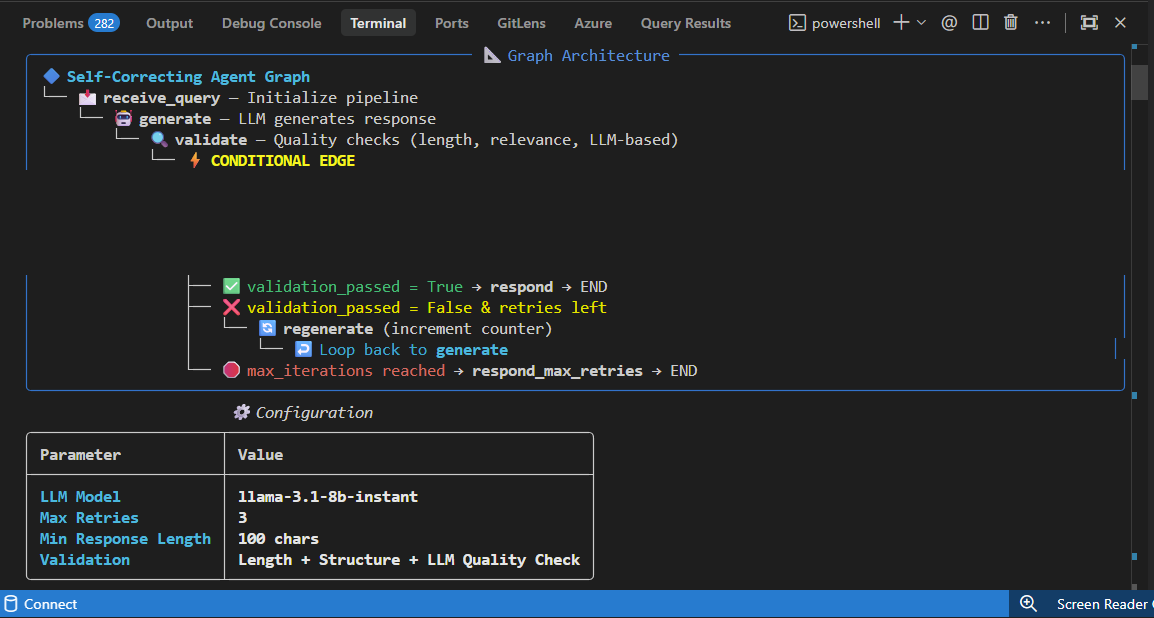
\includegraphics[width=\linewidth]{screenshots/Week4/Lab4.2-1.png}
        \caption{Agent Loop Architecture}
    \end{minipage}\hfill
    \begin{minipage}{0.31\textwidth}
        \centering
        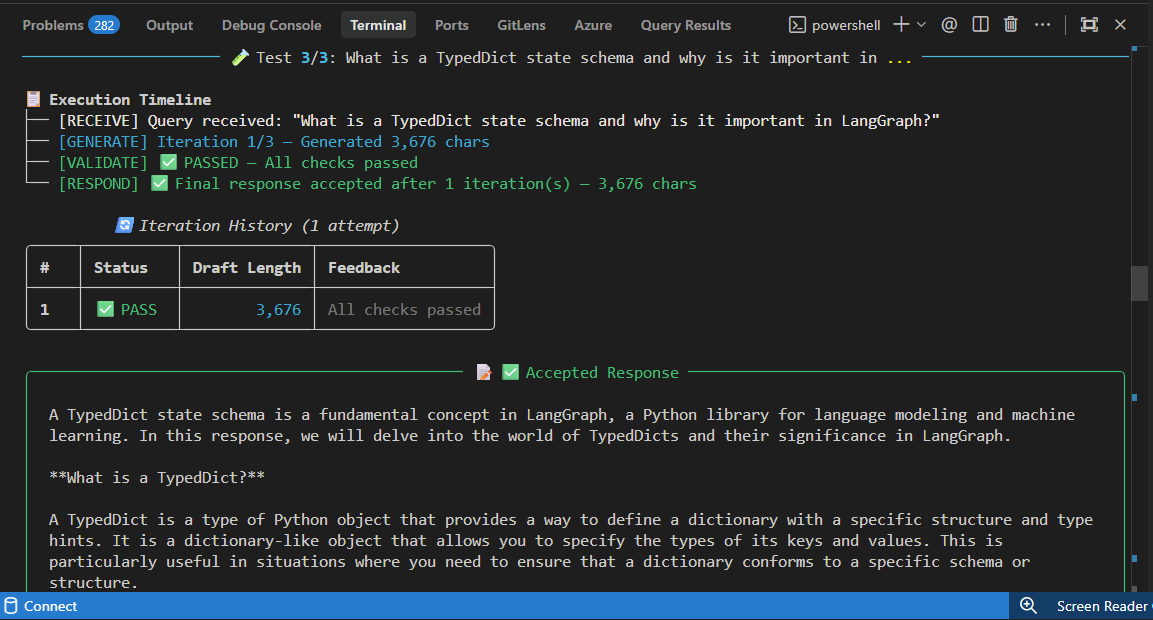
\includegraphics[width=\linewidth]{screenshots/Week4/Lab4.2-2.png}
        \caption{Iteration Tracking \& Final Output}
    \end{minipage}\hfill
    \begin{minipage}{0.31\textwidth}
        \centering
        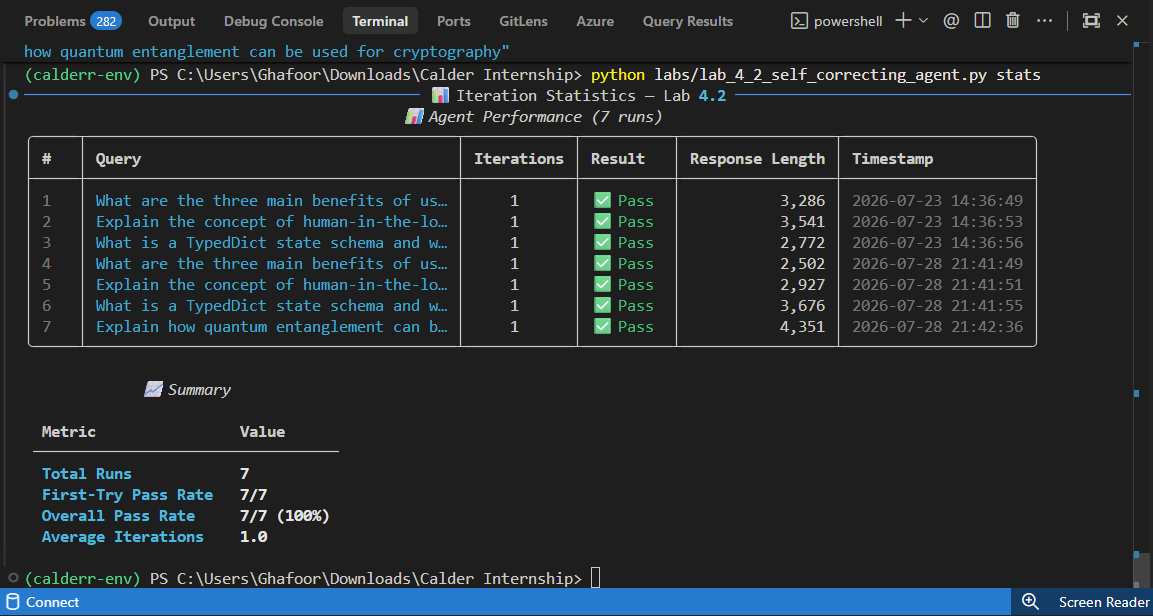
\includegraphics[width=\linewidth]{screenshots/Week4/Lab4.2-3.png}
        \caption{Agent Performance \& Summary}
    \end{minipage}
\end{figure}

\newpage

\subsection{Lab 4.3: Human-in-the-Loop Approval Workflow}
Engineered a sophisticated content moderation pipeline demonstrating robust state persistence.
\begin{itemize}[label=\textcolor{secondary}{$\bullet$}]
    \item \textbf{Moderation Routing:} Posts dynamically flow through auto-approve, borderline human review, or auto-reject stages based on initial scoring.
    \item \textbf{State Persistence:} Proved that the graph state correctly persists across the human review interrupt, safely resuming the workflow upon a manual decision.
\end{itemize}

\begin{figure}[H]
    \centering
    
\includegraphics[width=0.85\textwidth]{"labs/Lab 4.3_Arch-Diagram.png"}
    \caption{Lab 4.3: LangGraph State Machine Architecture}
\end{figure}

\begin{figure}[H]
    \centering
    \begin{minipage}{0.48\textwidth}
        \centering
        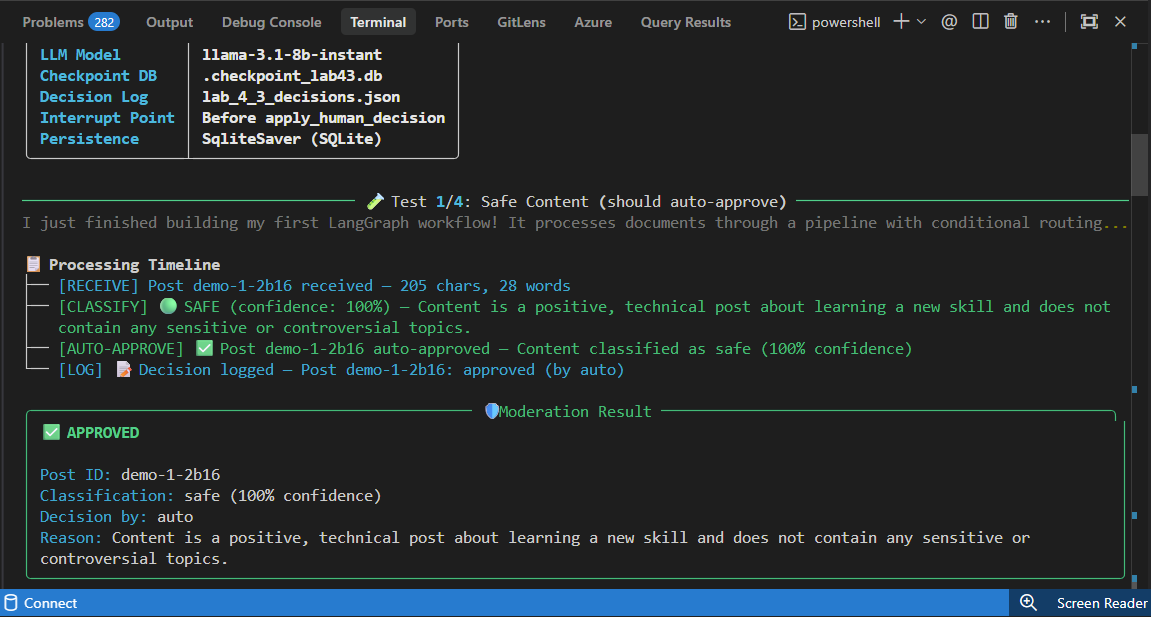
\includegraphics[width=\linewidth]{screenshots/Week4/Lab4.3-1.png}
        \caption{Moderation Routing Logic}
    \end{minipage}\hfill
    \begin{minipage}{0.48\textwidth}
        \centering
        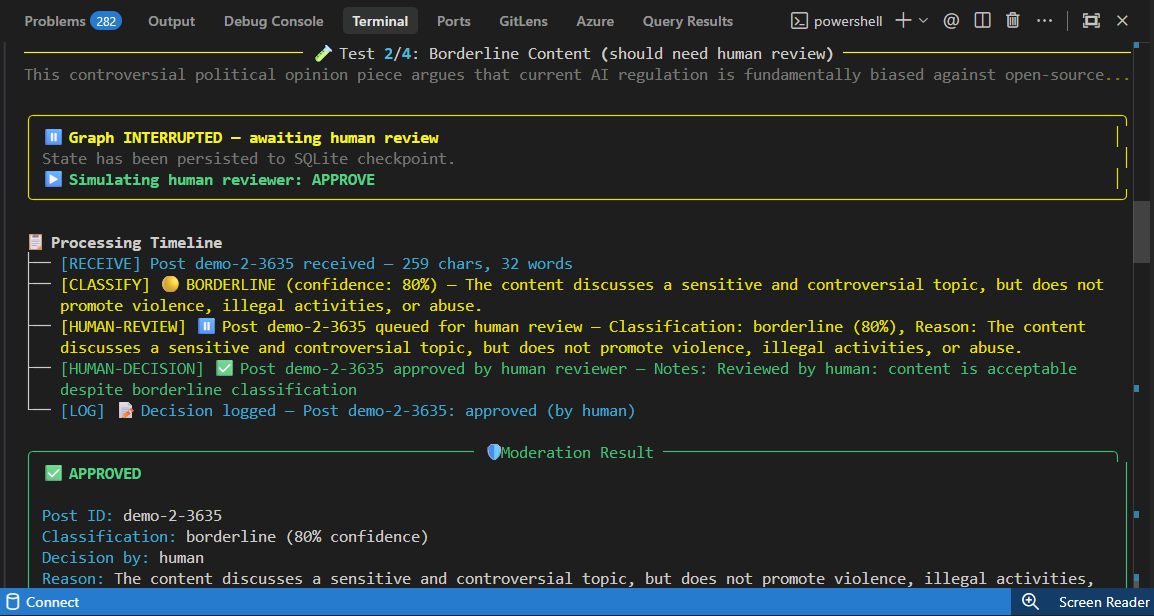
\includegraphics[width=\linewidth]{screenshots/Week4/Lab4.3-2.png}
        \caption{Borderline Post Triggering Interrupt}
    \end{minipage}
\end{figure}

\begin{figure}[H]
    \centering
    \begin{minipage}{0.48\textwidth}
        \centering
        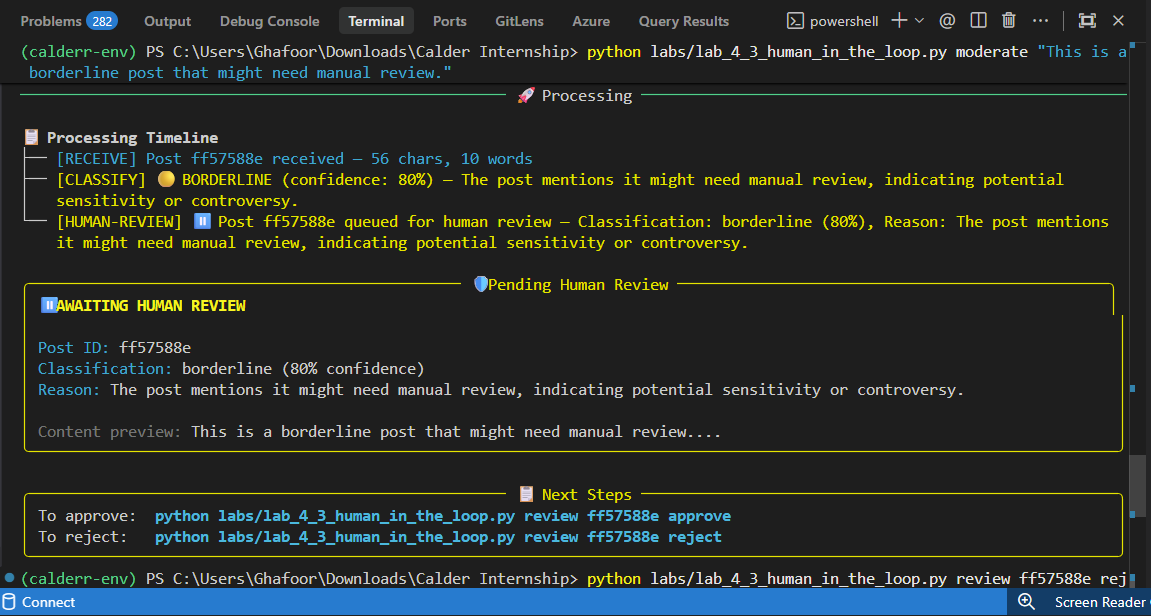
\includegraphics[width=\linewidth]{screenshots/Week4/Lab4.3-3.png}
        \caption{Human Review Action \& Resumption}
    \end{minipage}\hfill
    \begin{minipage}{0.48\textwidth}
        \centering
        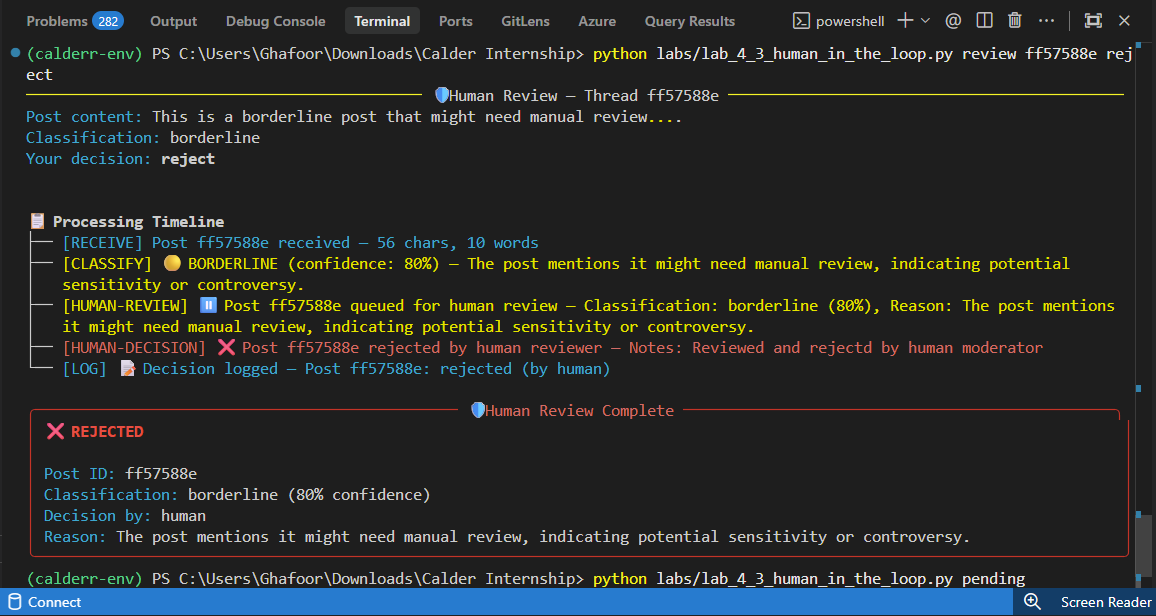
\includegraphics[width=\linewidth]{screenshots/Week4/Lab4.3-4.png}
        \caption{State Persistence \& Final Decision}
    \end{minipage}
\end{figure}

\vspace{0.5cm}

% --- Conclusion ---
\section{Conclusion \& Next Steps}
Week 4 successfully transitioned our capabilities from linear chains into highly robust, stateful, and dynamic agent architectures using LangGraph. By mastering node-edge graphs, conditional routing, human-in-the-loop approvals, and state persistence, the foundation has been laid for building complex, real-world AI systems that can reason, self-correct, and collaborate with humans over extended periods.

\end{document}
